\documentclass[a4paper,10pt]{article}

\usepackage{mathptmx}
\usepackage{helvet}
\usepackage{courier}
\usepackage{type1cm}
\usepackage{graphicx}

\usepackage[ngerman]{babel}
\usepackage{ngerman}
\usepackage[T1]{fontenc}
\usepackage[utf8]{inputenc}
\usepackage[fleqn]{amsmath}

\usepackage{color, enumerate, graphicx,booktabs,hyperref}
\usepackage[fleqn]{amsmath}

\setlength{\parindent}{0pt} %kein Einzug beim Absatzbegin

\begin{document}
	\title{Zusammenfassung: Interaktive Systeme}
	\author{Jannik Arndt}
	\date{Sommersemester 2012}
	\maketitle
	\tableofcontents

\pagebreak

\section{Die geschichtliche Entwicklung des Feldes HCI}
$\rightarrow$ \url{http://www.slideshare.net/mrettig/interaction-design-history}
\par
Grober Verlauf:
\begin{itemize}
	\item Use the Machine
	\item Use the Software
	\item Perform a Task
	\item Experience
	\item Connect
	\item Dynamically Enable
\end{itemize}

\section{Beispiel: OLB Baunfinanzierung}
\subsection{Ansätze}
\begin{enumerate}
	\item Interview mit einem Stakeholder
	\item Paper-/Wireframe-Prototyping
	\item Open Card Sorting
\end{enumerate}

\subsection{Iterative Design Phase}
\begin{enumerate}
	\item Cognitive Walkthrough
	\item Usability-Test
\end{enumerate}

\section{User Requirements}
Was macht Projekte erfolgreich?
\begin{itemize}
	\item User Involvement
	\item Clear Statement of Requirements
\end{itemize}

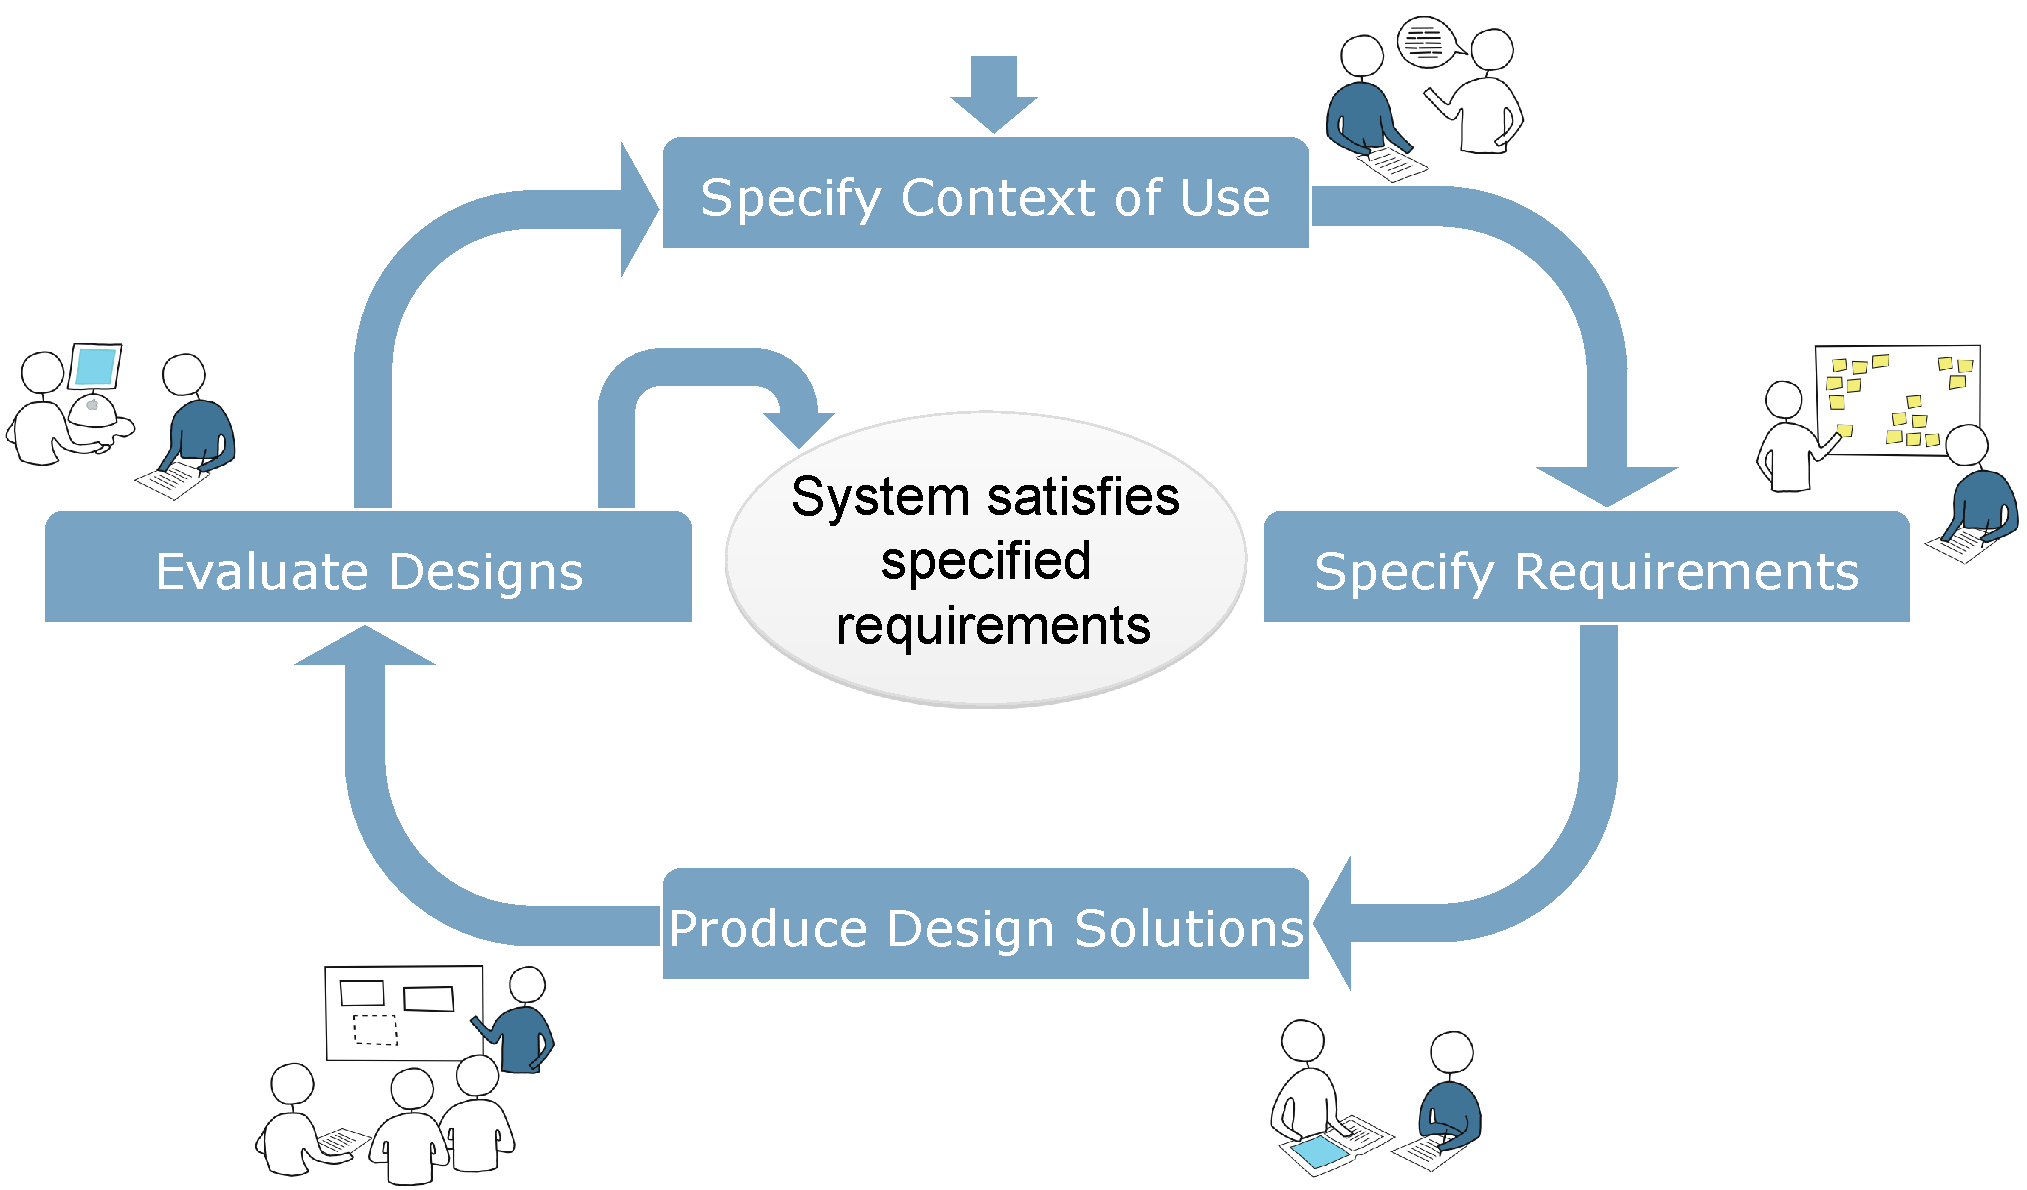
\includegraphics[width=\textwidth]{inc/HCDP.pdf}

\subsection{Context of use analysis}
\begin{itemize}
	\item Wer wird das System benutzen?
	\item Wer hat außerdem Interesse daran, dass alles läuft?
	\item Welche Charakteristiken haben diese Gruppen?
	\item Wie werden Vorgänge normalerweise ausgeführt?
	\item Umgebungen:
	\begin{itemize}
		\item technisch: Hardware, Software
		\item physikalisch: Wetter, Beleuchtung, ...
		\item sozial: Arbeitsweisen, Organisationsstrukturen, Einstellungen
	\end{itemize}
\end{itemize}

\subsection{Umfragen}
\subsubsection{Fragebögen}
\begin{itemize}
	\item Oft für statistischen Nutzen
	\item Antwortmöglichkeiten:
	\begin{itemize}
		\item Ja / Nein-Boxen
		\item Mehrere Optionen
		\item Likert-Skala (Grad der Zustimmung)
		\item Offene Fragen
	\end{itemize}
	\item Vorteile:
	\begin{itemize}
		\item Zeit- und Kosteneffizient
		\item Inhaltlich frei
		\item Relativ fehlerfrei wenn standardisiert
		\item Einfach zu verwalten
	\end{itemize}
	\item Nachteile:
	\begin{itemize}
		\item Ergebnis hängt stark vom Befragten ab
		\item Vorauswahl dadurch, dass die TN eventuell nicht repräsentativ sind
	\end{itemize}
\end{itemize}

\subsubsection{Interviews}
\begin{itemize}
	\item Strukturiert (weniger Kontextinformationen, einfacher zu interpretieren)
	\item Semi-strukturiert
	\item Offen (abhängig vom Können des Interviewers)
	\item Vorteile:
	\begin{itemize}
		\item Einfach, effizient und praktisch
		\item Hohe Validität
		\item Nachfragen möglich
		\item Einfach aufzunehmen
	\end{itemize}
	\item Nachteile:
	\begin{itemize}
		\item Abhängig vom Können des Interviewers
		\item Interviewer könnte Antworten beeinflussen
		\item Zeitaufwändig und teuer
		\item Nicht verlässlich
		\item Ergebnisse sind schwierig zu verallgemeinern
	\end{itemize}
\end{itemize}


\subsubsection{Zielgruppen}
\begin{itemize}
	\item 6--12 Teilnehmer
	\item Konzentration auf ein Thema, $\rightarrow$ Gruppendiskussion
	\item Ideen erzeugen, Produkte vergleichen, ...
	\item Heterogenität ist nützlich, aber nicht über Hierarchien oder in gengnesätzlichen Ansichten
	\item Vorbereitung:
	\begin{itemize}
		\item Zeit einplanen (1--3 Stunden)
		\item Fragen vorbereiten (4--10)
		\item TN einladen und Ziele erklären
		\item Material bereitstellen
	\end{itemize}
	\item Vorteile:
	\begin{itemize}
		\item Breit gestreute und qualitative Informationen
		\item Zeigt Konfliktpotenzial auf
		\item Günstig und einfach
	\end{itemize}
	\item Nachteile:
	\begin{itemize}
		\item Teilnehmer sind nicht repräsentativ
		\item Rolle des Moderators ist groß
		\item Einzelne TN können dominieren
		\item Nicht quantitativ
		\item Schwer zu verallgemeinern
	\end{itemize}
\end{itemize}

\subsection{Ethnographische Studien}
\begin{itemize}
	\item Beobachtung von Menschen im Supermarkt, zu Hause, bei der Arbeit, ...
	\item Ziel: Verhalten verstehen
	\item Aufzeichnungen mit Papier und Stift / Audio und Video / Computerlogging / Tagebuch (vom TN geschrieben)
	\item Tagebuch:
	\begin{itemize}
		\item Informationen zu Ort, Zeit, was passiert ist
		\item Alternativ zum Schreiben: Diktiergerät, Kamera, E-Mail-Adresse, ...
		\item Hinterher intensives Interview
		\item Vorteile:
		\begin{itemize}
			\item Billig
			\item Über längere Dauert möglich
			\item Gut für Nutzungskontext
		\end{itemize}
		\item Nachteile:
		\begin{itemize}
			\item Hängt von Motivation ab
			\item Nicht verlässlich
		\end{itemize}
	\end{itemize}
\end{itemize}

\subsection{Task Analysis}
\begin{itemize}
	\item Möglichkeiten für neue Produkte finden
	\item Task-decomposition: abstraktere Aufgaben in Teilaufgaben unterteilen
\end{itemize}

\subsection{Studien durchführen}
\begin{itemize}
	\item Informationsblatt und Einverständniserklärung sind wichtig
	\item Guidelines:
	\begin{enumerate}
		\item Wünsche des Stakeholders erfassen
		\item Alle Stakeholder beachten
		\item Mehr als einen Repräsentaten jeder Stakeholder-Gruppe
		\item Datenerhebungstechniken kombinieren
		\item Unterstützung durch Prototypen oder Aufgabenbeschreibungen
		\item Pilotstudie durchführen
		\item Daten aufnehmen
		\item Zeitnah mit der Interpretation beginnen
		\item Interpretation vor der Analyse (WTF?!)
	\end{enumerate}
\end{itemize}

\subsection{Anforderungsspezifikation}

\subsubsection{Personas}
\begin{itemize}
	\item Fiktionale Repräsentation eines typisches Nutzers
	\item Hintergrundinformationen aus Literatur, Interviews, Beobachtungen, Statistiken
	\item Repräsentativ aber nicht durchschnittlich
\end{itemize}

\subsubsection{Szenarien}
Erzählerische Beschreibung eines Anwendungsfalls, betrachtet dabei auch den Kontext des Benutzers.

\subsubsection{Anwendungsfälle}
Aus dem Software Engineering, Interaktion mit der Funktionalität eines Systems.

\subsection{Vorwissen}

\subsubsection{State of the Art Analysis}
Vergleich von existierenden Systemen.

\subsubsection{General Design Principles}
Beispiele:
\begin{itemize}
	\item Shneiderman‘s „Eight Golden Rules of Dialog Design“
	\item ISO9241: Accessibility and Usability
	\item Mayhew‘s General Principles of User Interface Design
	\item IBM‘s Design Principles for tomorrow
	\item Platform guidelines
	\item Corporate Design guidelines
\end{itemize}

\section{UI Structure and Design}

\subsection{Einführung}
\subsubsection{Zielgruppe}
\begin{itemize}
	\item Demographische Einschätzung (Alter, Geschlecht, Ort, Bildung, Arbeit, Einkommen, Hobbys, Ausstattung, ...)
	\item Einschätzung nach Erfahrung und Verhalten (Anfänger, Fortgeschritten, Experte, ...)
\end{itemize}

\subsubsection{Ziele}
\begin{itemize}
	\item Ziele der Anwendung (Unterhaltung, Bildung, Büro, Verwaltung, Kommunikation, Information, ...)
	\item Ziele der Benutzer (Wissen erlangen, einen Freund erreichen, ein Problem lösen, ein Dokument erstellen, ...)
\end{itemize}

\subsubsection{Inhalt}
\begin{itemize}
	\item ???
\end{itemize}

\subsection{Strukturdesign}
\subsubsection{Struktur}
\begin{itemize}
	\item Hierarchien sind einfach
	\item Ordnen nach Wichtigkeit, Granularität, Erwartungen, Bedürfnissen
	\item Lieber in die Breite als in die Tiefe gehen
	\item Maximale Tiefe: 5--6 Level
\end{itemize}

\subsubsection{Ausrichtung und Navigation}
\begin{itemize}
	\item Benutzerfragen:
	\begin{itemize}
		\item Wo bin ich? $\rightarrow$ Brotkrumen-Navigation
		\item Was kann ich tun? $\rightarrow$ Beware the big button trap (???)
		\item Was passiert wenn ich dies tue?
		\item Wo komme ich her? / Wie komme ich zurück?
	\end{itemize}
	\item Visuelles (Farben, Schriften, Bilder und Symbole) sollten einfach leicht zu merken sein
	\item Ein Menü ist gut für Navigation und Orientierung
	\item Weißraum: Trennt Informationen, hebt hervor
\end{itemize}
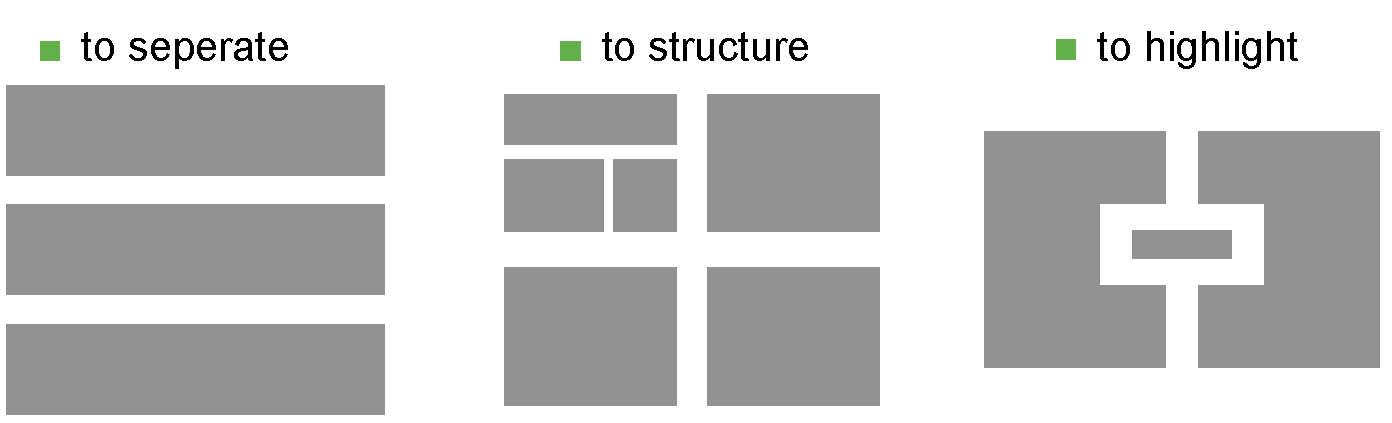
\includegraphics[width=\textwidth]{inc/whitespace.pdf}

\subsubsection{Card Sorting}
\begin{itemize}
	\item Man fragt die Benutzer, wie sie Inhalt strukturieren und benennen würden
	\item Dabei werden Muster (=\emph{Mentale Modelle}) gesucht
	\item Gut geeignet für Menü-Kategorien und Navigation
	\item Methode:
	\begin{itemize}
		\item Inhalt vorauswählen, auf ähnliche Granularität (Detaillevel) achten
		\item Ungefähr 30 Karten
		\item Kurze, schnell zu lesende aber aussagekräftige Begriffe
		\item Freie Karten um Begriffe zu ergänzen
	\end{itemize}
	\item Durchführung:
	\begin{itemize}
		\item Teilnehmer sollten repräsentativ sein
		\item TN einzeln (15--30 TN) oder in 5 Gruppen à 3 TN
		\item Material: beschriftete und freie Karten, Stift, Gummibänder, Büroklammern, Klebstoff
		\item Am Anfang Einführung geben, dann beobachten
	\end{itemize}
	\item Analyse:
	\begin{itemize}
		\item Muster durch Ordnung auf dem Tisch, am Whiteboard, ...
		\item Unterschiede deuten auf fehlendes oder falsches Verständnis hin
		\item Methoden: Multidimensional Scaling, Hierarchical Cluster Analysis
	\end{itemize}
\end{itemize}

\subsection{Bildschirmdesign und -layout}
\subsubsection{Gestaltgesetze}
\begin{itemize}
	\item Köhler, Koffka, Werheimer (Berliner Schule), 1912: Gestaltpsychologie
	\item Basiert auf Wahrnehmung, Bewegung, Gedächtnis, Denken, Lernen und Verhalten
	\item Insgesamt über 100 Gesetze
\end{itemize}

\begin{enumerate}
	\item Prägnanz: Einfache Formen
	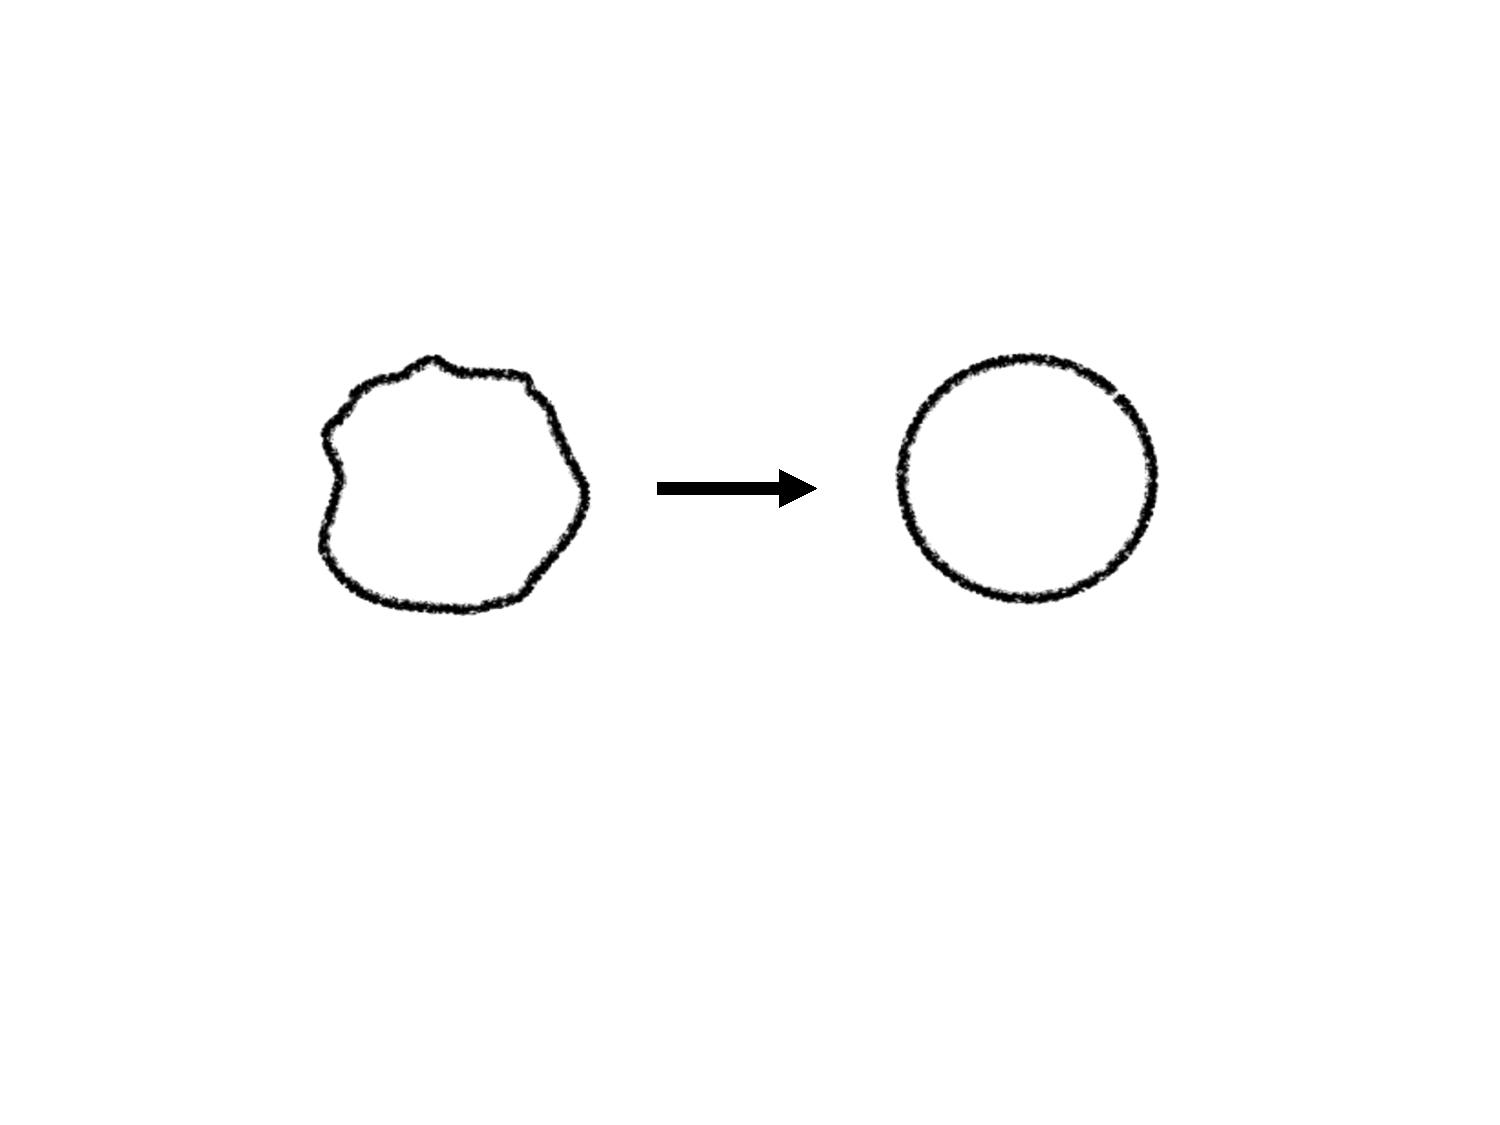
\includegraphics[width=4cm]{inc/gestalt_1.pdf}
	\item Nähe: Beieinander liegende Objekte sind zusammengehörig
	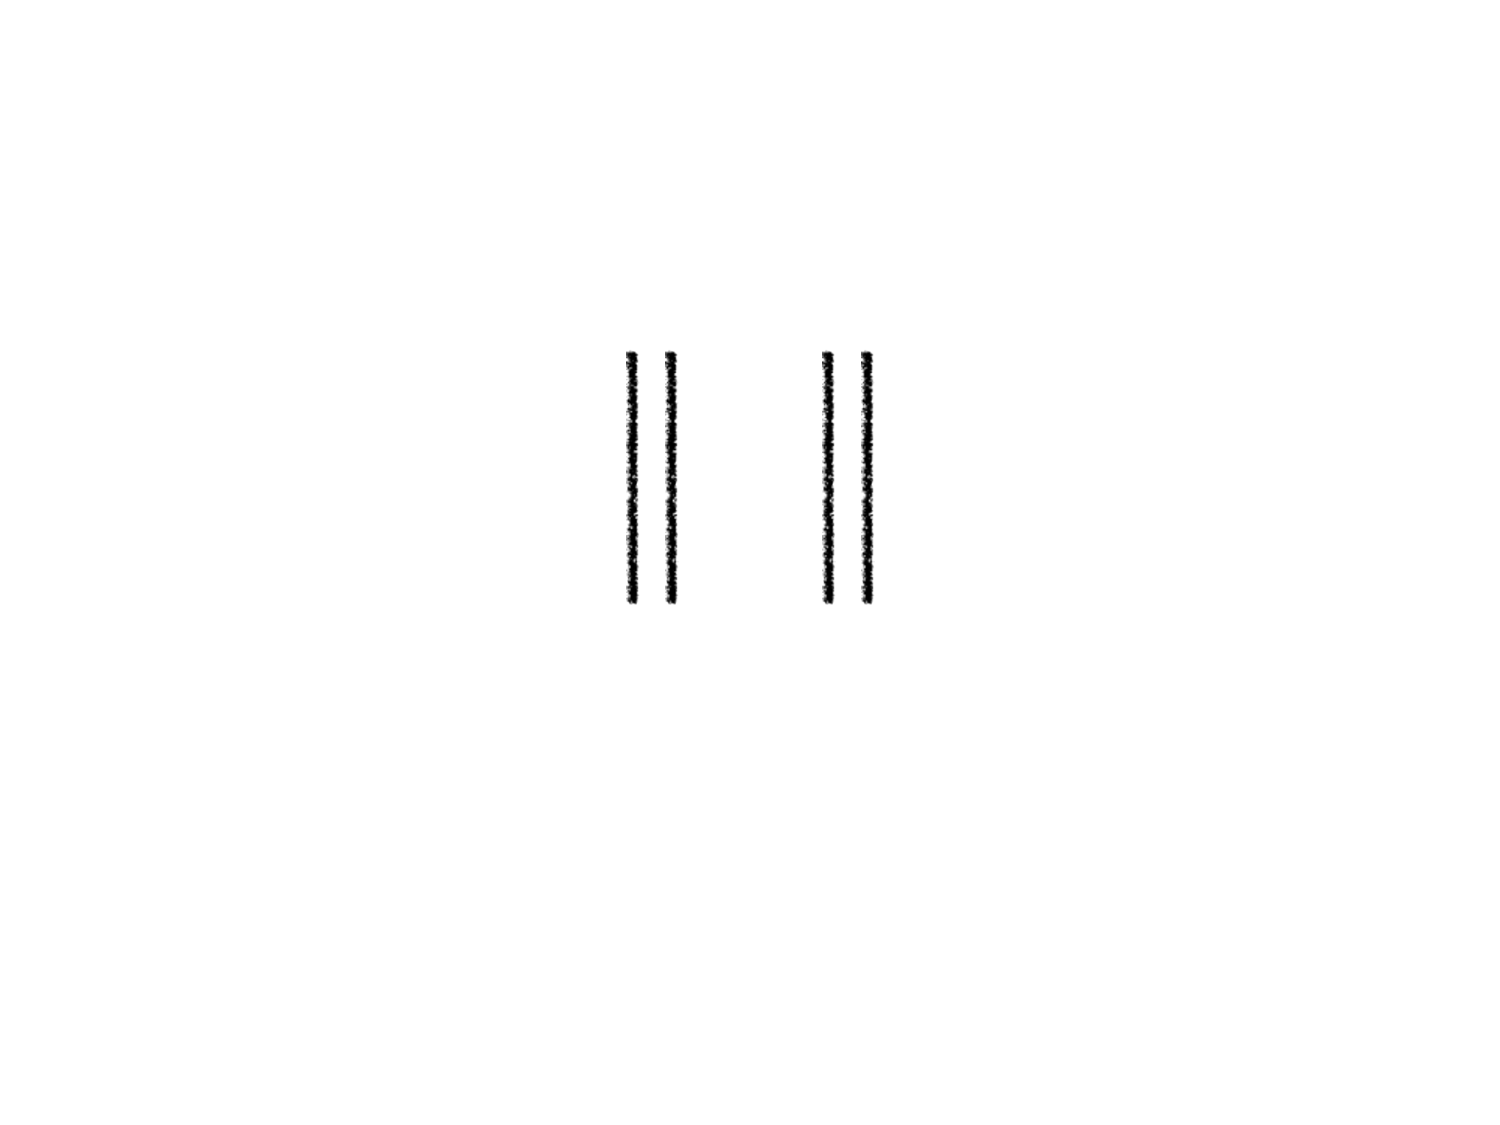
\includegraphics[width=2cm]{inc/gestalt_2.pdf}
	\item Geschlossenheit: Fenster-Metapher
	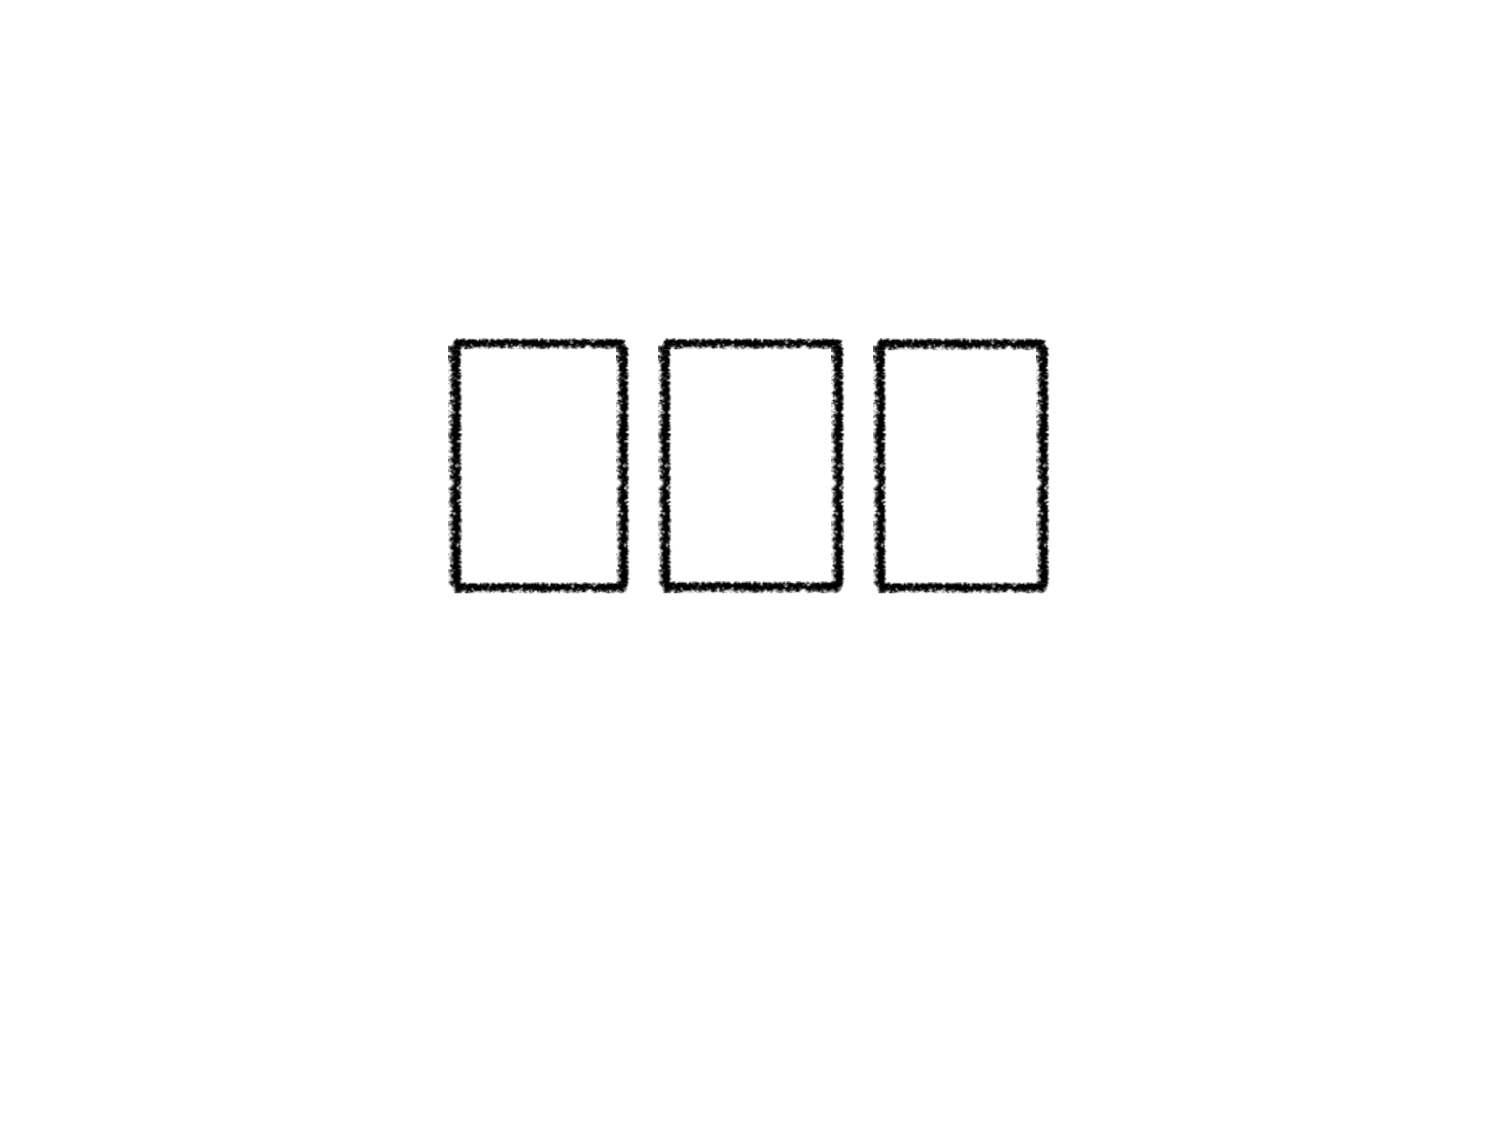
\includegraphics[width=4cm]{inc/gestalt_3.pdf}
	\item Ähnlichkeit: Ähnliche Formen gehören zusammen
	
\includegraphics[width=2cm]{inc/gestalt_4.pdf}
	\item Gute Fortsetzung: Kontinuierliche Formen gehören zusammen
	
\includegraphics[width=3cm]{inc/gestalt_5_1.pdf}
	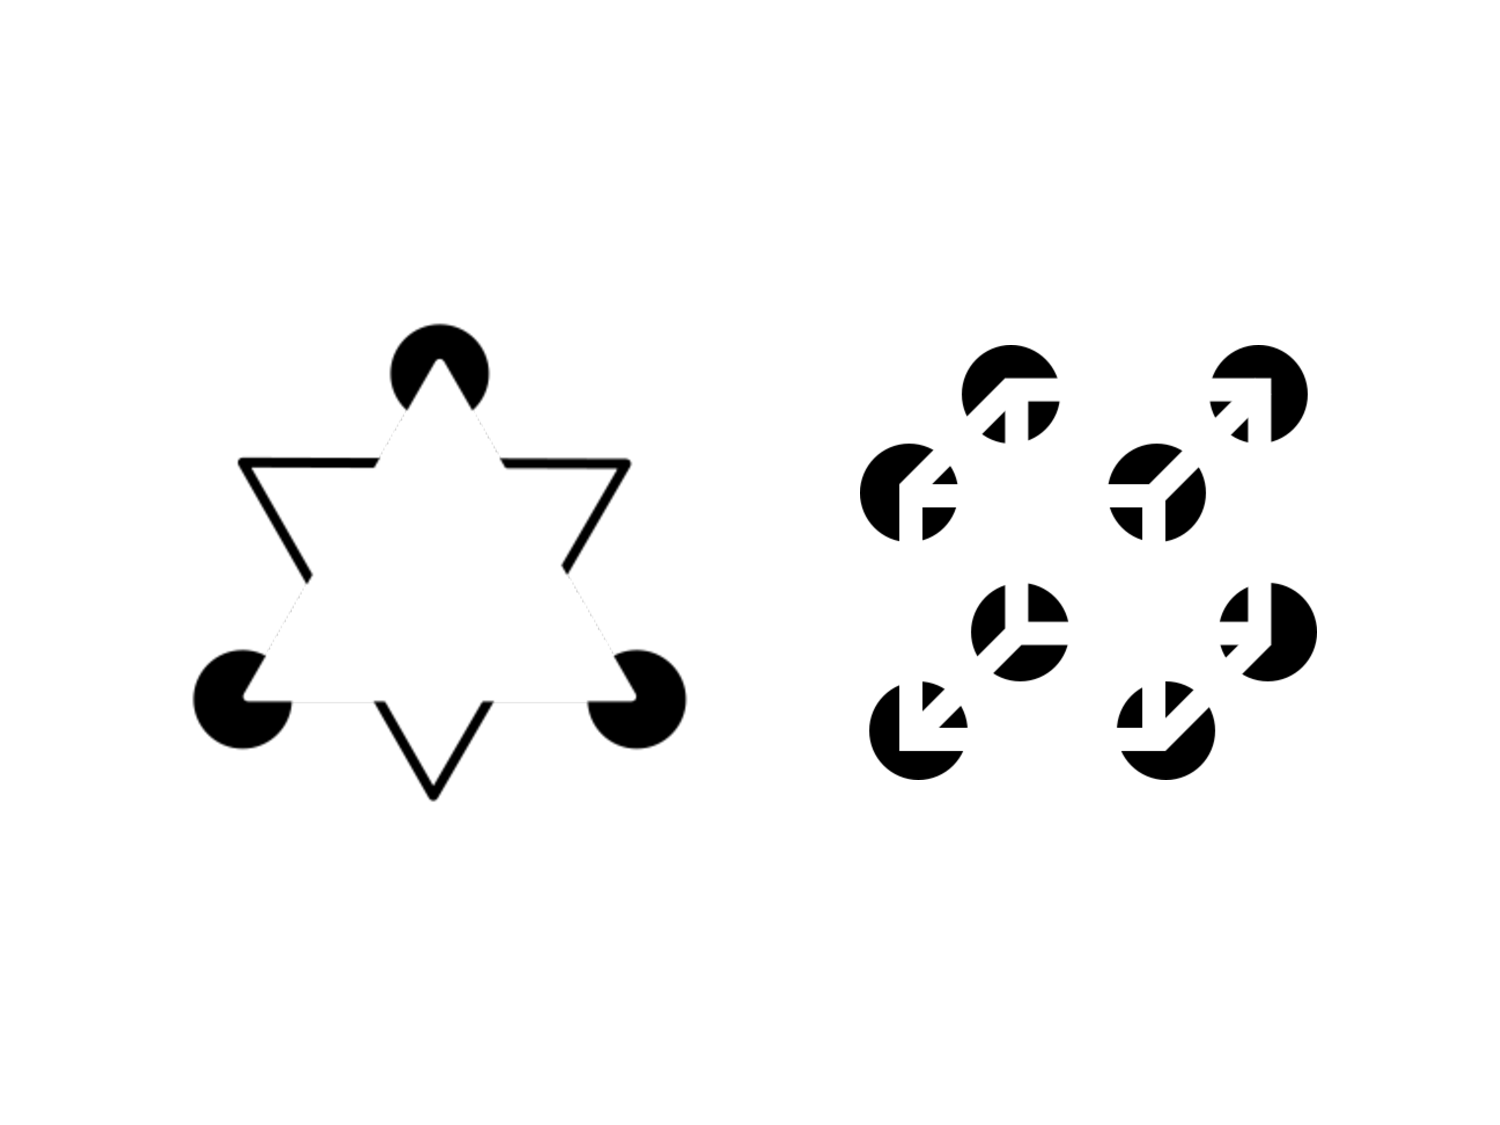
\includegraphics[width=4cm]{inc/gestalt_5_2.pdf}
	\item Erfahrung: Neue Informationen werden in bekannte Strukturen eingeordnet
	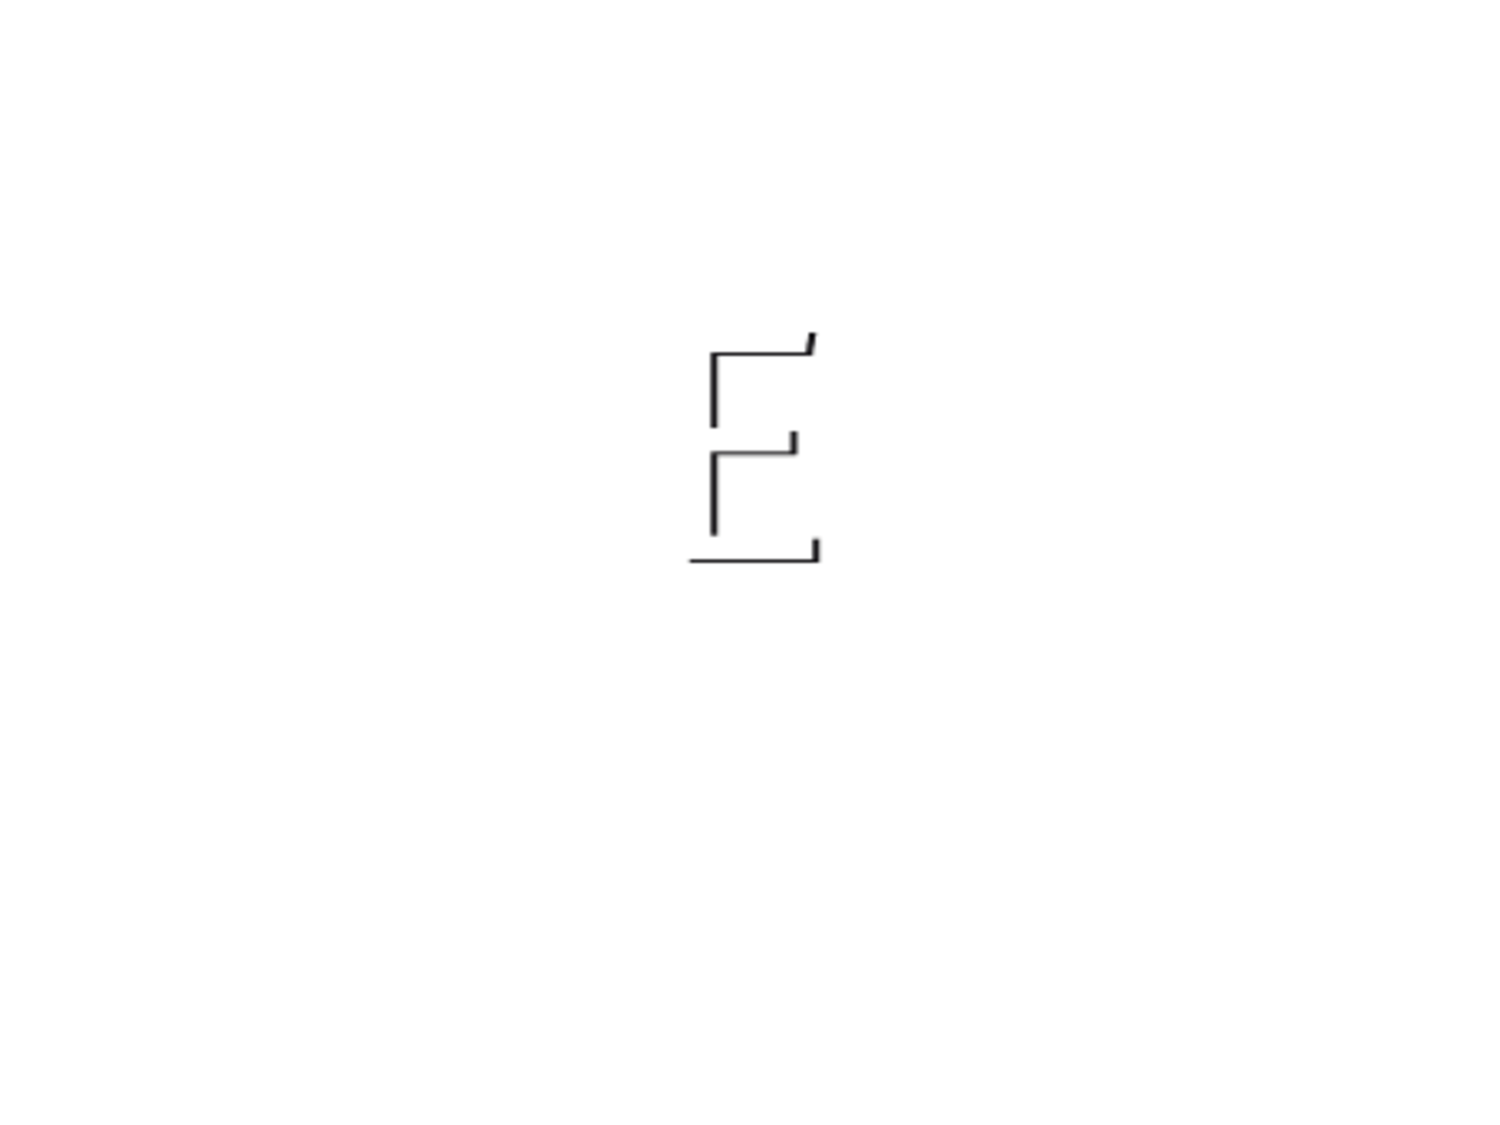
\includegraphics[width=1cm]{inc/gestalt_6.pdf}
	\item Gemeinsame Bewegung:
	
\includegraphics[width=2cm]{inc/gestalt_7.pdf}
\end{enumerate}

\subsubsection{Farben}
\begin{itemize}
	\item Farben sind nie neutral, können Emotionen hervorrufen und sind oft unterbewusst wahrgenommen
	\item Einflüsse: Biologisch, Kulturell, Individuell
	\item Benachbarte Farben beruhigen
	\item Komplementäre Farben erzeugen Spannung
	\item Maximal 4--5 Farben benutzen
	\item Farben konsistent benutzen
\end{itemize}

\subsubsection{Bilder und Symbole}
\begin{itemize}
	\item Illustration, Dekoration, Strukturierung
	\item Bilder
	\begin{itemize}
		\item sparen Platz,
		\item sind leicht zu erkennen,
		\item Sprachunabhängig,
		\item einfach zu merken,
		\item unterbewusst wahrnehmbar
	\end{itemize}
	\item Gute Bilder
	\begin{itemize}
		\item zeigen nur das wichtigste,
		\item kombinieren Bekanntes mit Neuem
		\item sprechen Emotionen an
	\end{itemize}
\end{itemize}

\subsubsection{Typographie}
\begin{itemize}
	\item strukturiert und hebt hervor
	\item beinhaltet Schriftart, Schriftschnitt, Größe, Farbe und Dekoration
\end{itemize}

\subsection{Keep in Mind}
Think from a user's perspective
\begin{itemize}
	\item When, where and how will they use the system?
	\item What are their characteristics?
	\item Are they handicapped?
	\item What do they expect?
	\item What are they accustomed to?
	\item What do they like?
\end{itemize}
Design for the actual users

\section{Gedächtnis und Aufmerksamkeit}
\begin{itemize}
	\item Geteilte Aufmerksamkeit: Auf alles gleichzeitig achten (z.B. Autofahren)
	\item Selektive Aufmerksamkeit: Konzentration auf einzelnes
	\item Methoden:
	\begin{itemize}
		\item Eyetracking
		\item Saliency Maps (Aufmerksamkeitskarten)
	\end{itemize}
\end{itemize}

\section{Affordance, Constraints, Models und Metaphern}

\subsection{Affordanzen}
\begin{itemize}
	\item Angebotscharakter: “An affordance is a quality of an object, or an environment, which allows an individual to perform an action.”
	\item Beispiel: Türen
\end{itemize}

\subsection{Mappings}
\begin{itemize}
	\item Verbindung zwischen Userinterface und echter Welt
	\item Gut: physikalische Analogie, kulturelle Standards
	\item Beispiele: räumlich, wahrnehmbare Analogien (Schalter sieht genauso aus, wie das, was er bedient)
\end{itemize}

\subsection{Constraints}
\begin{itemize}
	\item Einschränkungen sind das Gegenteil von Affordanzen und können diese Vergrößern
	\item Ziel: Benutzungsfehler vermeiden, Information, die erinnert werden muss, reduzieren
	\item Arten:
	\begin{itemize}
		\item Physikalisch: Schränken physische Operationen ein, z.B. durch eine Form
		\item Semantisch: Sich aus dem Kontext und dem Wissen über die Welt ergebene Einschränkungen
		\item Logisch: Das, was logisch erscheint
		\item Kulturell: Farben oder Schriften-abhängig
	\end{itemize}
\end{itemize}

\subsection{Konzeptuelle Modelle}
\begin{itemize}
	\item Modelle sorgen dafür, dass nicht über jede Handlung nachgedacht werden muss, sondern Dinge automatisch erledigt werden können.
\end{itemize}

\subsection{Metaphern}
\begin{itemize}
	\item Ein Bekannter Begriff wird als Analogie zu einem unbekannten Sachverhalt verwandt
	\item Gefahr der Unter-/Überschätzung des Systems durch zu genaue Analogie
	\item Reduktion auf Kernmerkmale
\end{itemize}

\section{Usability Guidelines}

\begin{itemize}
	\item Definition: “The extent to which a product can be used by specified users to achieve specified goals with effectiveness, efficiency and satisfaction in a specified context of use.” [ISO 9241-11]
	\item Unterschied: Effektivität (ein Ziel erreichen) und Effizienz (ein Ziel mit minimalem Aufwand erreichen)
	\item Leaky Pipe Metaphor: Auf dem Weg zum Ziel werden Benutzer verloren (“Drop outs”), weil sie das Interface nicht richtig bedienen
	\item Vorteile guter Usability:
	\begin{itemize}
		\item gesteigerte Produktivität
		\item Glückliche Benutzer
		\item Weniger Kosten (Zeit, Geld, Gesundheit) (?)
	\end{itemize}
	\item Es gibt Theorien, Prinzipien und Richtlinien (abstrakt nach konkret):
\end{itemize}

\subsection{Theorien}
\begin{itemize}
	\item Kognition: GOMS, ACT-R
	\item Sinne: Sehen, Hören, Fühlen
	\item Bewegung: Fitts' Law
\end{itemize}

\subsubsection{Fitts' Law}
\begin{itemize}
	\item Modell für die motorische Bewegung
	\item Besonders für schnelles Zielen
	\item Beschreibendes und vorhersehendes Modell
	\item Die Schwierigkeit einer Bewegung ist abhängig von der \emph{zurückzulegenden Distanz} und der \emph{Größe des Ziels}
	\item Kanten und Ecken sind am Besten zu erreichen
\end{itemize}

\subsection{Prinzipien}
\begin{itemize}
	\item Shneiderman's 8 Golden Rules of Interface Design
	\item Niesen's 10 Heuristics for User Interface
	\item Tognazzini's First (16) Principles of Interface Design
\end{itemize}

\subsubsection{8 Goldene Regeln für Interface Design}
\begin{enumerate}
	\item Konsistenz: Reihenfolge von Handlungen, Begriffe, Design
	\item Universale Usability: Menschen sind unterschiedlich
	\item Informative Rückmeldung: für \emph{jede} Handlung muss es Feedback geben
	\item Abschließen von Dialogen: Nach Beendigung einer Aufgabe muss es abschließendes Feeback geben
	\item Fehler verhindern: z.B. falsche Eingaben
	\item Einfaches Rückgängig machen: gibt dem Benutzer Sicherheit
	\item Benutzerkontrolle: Der Benutzer sollte immer die Kontrolle haben
	\item Kurzzeitgedächtnis entlasten: es können nur etwa 7 $(\pm2)$ “Datenpakete” gemerkt werden
\end{enumerate}

\subsection{Richtlinien}
\begin{itemize}
	\item Finden sich z.B. oft in Betriebssystemen
\end{itemize}
\begin{enumerate}
	\item Navigation: Linktext sollte immer aussagekräftig sein, Überschriften eindeutig und beschreibend
	\item Organisation der Anzeige: Datenformate sollten einheitlich und bekannt sein, Eingabe sollte Anzeige entsprechen, Ausgabe sollte editierbar sein
	\item Aufmerksamkeit erlangen:
	\begin{itemize}
		\item 2 Stufen Instensität (Fettdruck)
		\item Unterstreichungen oder Pfeile
		\item Bis zu 4 Schriftgrößen
		\item Bis zu 3 Schriftarten
		\item Kein Blinken
		\item Bis zu 4 Farben
		\item Sanfte Töne = gut / Harte Töne = Fehler
	\end{itemize}
\end{enumerate}


\subsection{Standards}
\subsubsection{ISO 9241}
Dialogprinzipien nach ISO 9241-110:
\begin{enumerate}
	\item Angemessenheit: Der Dialog sollte den Nutzer unterstützen
	\item Selbsterklärung: entweder sofort verständlich oder auf Anfrage mit Hilfe versehen
	\item Kontrollierbarkeit: Der Benutzer kontrolliert, nicht der Computer
	\item Übereinstimmung mit Erwartungen
	\item Fehlertoleranz: Fehler sollen mehr oder weniger automatisch behoben werden
	\item Möglichkeit der Individualisierung
	\item Lernmöglichkeiten
\end{enumerate}

\subsection{User Experience vs. Usability}

User Experience = Usability + Motivation + Emotionen + Werte


\section{Prototyping}
\begin{itemize}
	\item Warum?
	\begin{itemize}
		\item Prototypen eignen sich für Nutzerstudien, den Nutzer wissen nicht, was sie wollen, sehr wohl aber was sie nicht wollen.
		\item Man kann Fragen beantworten (Funktioniert das Konzept?)
		\item Alternativen vergleichen
	\end{itemize}
	\item Wann?
	\begin{itemize}
		\item Je frühe, umso besser
	\end{itemize}
	\item Was?
	\begin{itemize}
		\item Alles
	\end{itemize}
	\item Ansätze
	\begin{itemize}
		\item Wegwerfprototypen (“rapid prototype”)
		\item Evolutionärerprototyp (wird weiterentwickelt)
		\item Inkrementeller Prototyp (ein Teil des Ganzen, wird später eingefügt)
		\item Horizontal (viele Features, wenig Funktionalität) $\leftrightarrow$ Vertikal (ein Feature, volle Funktionalität)
		\item Li-Fi-Prototype (früh, billig, oberflächlich) $\leftrightarrow$ Hi-Fi-Prototype (viele Details)
	\end{itemize}
	\item Techniken
	\begin{itemize}
		\item Storyboarding
		\item Paper-Prototype
		\item Click-Prototype (GUI, z.B. Pidoco)
		\item Wizard-Of-Oz-Prototype (Mensch ersetzt Funktionalität)
	\end{itemize}
\end{itemize}

\section{Usability Evaluation 1 --- Testing with Users}

\section{Usability Evaluation 2 --- Analytical and Expert Methods}





















\end{document}
